% Synchronized to r53967
\section {SSHD - Secure Shell, Secure Copy}

A secure shell enables you to open an encrypted connection with the fli4l router. 
By using secure copy files can be transmitted encrypted to the fli4l router. If 
in addition \jump{SSHDPUBLICKEYN}{Public Key Login} is used commands and file 
transfers can be executed driven by scripts from ``outside''. As of version 2.1.7 
only a SSH2 server is existing.

\subsection {Installation Of The Secure-Shell-Daemon}

\begin{description}

\config {OPT\_SSHD}{OPT\_SSHD}{OPTSSHD}

  Default setting: \var{OPT\_\-SSHD='no'}

  If the router should be accessible via ssh set \var{OPT\_\-SSHD} to \var{'yes'}. 
  This will install the ssh server Dropbear on the fli4l router. It will also 
  enable copying of files to the router.
  
\config {SSHD\_ALLOWPASSWORDLOGIN}{SSHD\_ALLOWPASSWORDLOGIN}{SSHDALLOWPASSWORDLOGIN}

  Default setting: \var{SSHD\_ALLOWPASSWORDLOGIN='yes'}

  If \var{SSHD\_ALLOWPASSWORDLOGIN} is set to \var{'no'} fli4l won't allow 
  ssh login via password anymore. Login can only be done via private/public key.
  This assumes that a \jump{SSHDPUBLICKEYN}{public key} is present 
  on the router.

\config {SSHD\_CREATEHOSTKEYS}{SSHD\_CREATEHOSTKEYS}{SSHDCREATEHOSTKEYS}

  Default setting: \var{SSHD\_CREATEHOSTKEYS='no'}

  A ssh server needs a so-called host key that is unique to identify itself 
  to a ssh client. The package SSHD provides a host key to allow a first 
  login to the router but this key should be replaced with a self-generated 
  one only known to you as fast as possible. Generating your own host key is 
  the only way to be prepared against so called man-in-the-middle attacks 
  and thus is very important. SSH will notice if someone pretends to be your 
  fli4l router because his host key will differ and will warn you about the 
  host key changing.
  
  Generating your own host key will be done automatically if 
  \var{SSHD\_CREATEHOSTKEYS} is set to \var{'yes'}. This is a challenging  
  task and can prolong boot time for several minutes. If the fli4l router 
  starts with \var{SSHD\_CREATEHOSTKEYS} activated one (or more) host key(s) 
  will be created in the directory \var{/tmp/ssh}. Keyfiles found there 
  have to be copied over to your fli4l build directory under \var{etc/ssh} 
  (on the PC where fli4l's boot medium is created). In my case a directory 
  listing of config.babel looks like this:

  \begin{figure}[htbp]
    \centering
    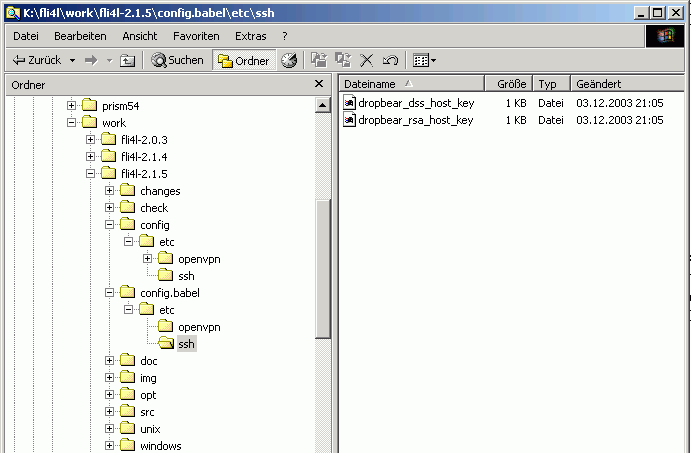
\includegraphics[width=\columnwidth]{etc_ssh_dir}
    \caption{Directory structure of fli4l}
    \label{fig:etc_ssh_dir}
  \end{figure}

  Please note that under the directory \var{config} a subdirectory 
  etc exists with another subdirectory ssh. Generated host keys have to 
  be placed there. As of fli4l version 2.1.5 files in your config directory 
  will be preferred over the ones from the opt directory. With the next 
  update of your fli4l boot medium the files from \var{config/etc/ssh}
  will be integrated and not those in \var{opt/etc/ssh}. In this way every 
  fli4l router you configure can have its own unique host key. When creating 
  the fli4l files there will appear a message \glqq{}appending config specific 
  files to opt.img ...\grqq{} towards the end. All files coming from the 
  config directory instead of opt will be listed there.

\begin{verbatim}
#
# appending config specific files to opt.img ...
#
etc/ssh/dropbear_dss_host_key
etc/ssh/dropbear_rsa_host_key
\end{verbatim}

  If you created a new host key set \var{SSHD\_\-CREATEHOSTKEYS} back to 
  \var{'no'} to avoid creating another host key on every reboot.

  If you log in to your fli4l router after updating the host key a warning 
  message (depending on the ssh client you use) will appear to inform you 
  about the changed host key. In this case this is normal because you just 
  changed your host key. Follow the routine necessary for your ssh client 
  to accept the changed host key permanently. If some time in the future 
  you see this warning again you will have to check why it appears. Don't 
  just accept a changed host key blindly!
  
\begin{verbatim}
@@@@@@@@@@@@@@@@@@@@@@@@@@@@@@@@@@@@@@@@@@@@@@@@@@@@@@@@@@@
@    WARNING: REMOTE HOST IDENTIFICATION HAS CHANGED!     @
@@@@@@@@@@@@@@@@@@@@@@@@@@@@@@@@@@@@@@@@@@@@@@@@@@@@@@@@@@@
IT IS POSSIBLE THAT SOMEONE IS DOING SOMETHING NASTY!
Someone could be eavesdropping on you right now (man-in-the-middle attack)!
It is also possible that the RSA host key has just been changed.
The fingerprint for the RSA key sent by the remote host is
ca:a4:ab:e7:af:d8:68:05:d3:1f:e6:15:08:d6:ed:36.
Please contact your system administrator.
Add correct host key in /home/babel/.ssh/known_hosts to get rid of this message.
Offending key in /home/babel/.ssh/known_hosts:7
Password authentication is disabled to avoid man-in-the-middle attacks.
\end{verbatim}

\config {SSHD\_PORT}{SSHD\_PORT}{SSHDPORT}
 
   Default setting: \var{SSHD\_PORT='22'}
 
   By \var{SSHD\_PORT} a non-standard port can be defined 
   the ssh server should listen to.
 
   If ssh login from outside should be allowed 
   \jump{PFNEWCONFIG}{\var{INPUT\_ACCEPT\_PORT\_x}} has to be adapted 
   to reflect the change.
 
   The commands accessing fli4l from an Unix-/Linux client over protocol SSH 
   are:
   \begin{itemize}
   \item ssh - Secure Shell
   \item scp - Secure Copy
   \end{itemize}
 
   Corresponding programs are available for Windows as well, see: \\
    \altlink{http://www.chiark.greenend.org.uk/~sgtatham/putty/} \\
    \altlink{http://winscp.net/eng/docs/lang:en} \\
    \altlink{http://www.tectia.com/de/de.iw3}

\config {SSHD\_PUBLIC\_KEY\_N}{SSHD\_PUBLIC\_KEY\_N}{SSHDPUBLICKEYN}

  Default setting: \var{SSHD\_PUBLIC\_KEY\_N='0'}

  \var{SSHD\_PUBLIC\_KEY\_N} holds the number of public keys to be 
  copied to the fli4l router.

  SSH allows authentification based on asymmetric encryption. 
  Authentification is done via username and public/private key 
  instead of username and password. This way entering a password 
  can be omitted. Generate your key pair by the help of ssh-keygen 
  (or puttygen if putty under Windows is used as the ssh client). 
  When generating keys you can optionally specify a passphrase 
  (a password for using the key) to increase security even more. 
  If using a passphrase you may consider working with an ssh agent 
  (ssh-agent or pageant).

  \wichtig{The private part of the keypair has to be guarded as careful 
  as a password because it has the same function. The private part 
  of your keypair is only known to your ssh client. The public part of the 
  key will be needed on the fli4l router and is provided to it by 
  \var{SSHD\_PUBLIC\_KEY\_x} or \var{SSHD\_PUBLIC\_KEYFILE\_x}.}

  For further informations see manual pages for ssh and its components 
  res. the documentation for putty
  (\altlink{http://www.chiark.greenend.org.uk/~sgtatham/putty/}).

\config {SSHD\_PUBLIC\_KEY\_x}{SSHD\_PUBLIC\_KEY\_x}{SSHDPUBLICKEYx}

  Provide the public part of each user's key here who should be 
  able to access flil4 via ssh. The easiest way is cut and paste it 
  from a terminal window. Example:

\begin{example}
\begin{verbatim}
        SSHD_PUBLIC_KEY_1='1024 ... username@hostname'
\end{verbatim}
\end{example}

 \wichtig{The key does not contain carriage returns. Puttygen will 
 insert those eventually while doing cut-and-paste. They will have 
 to be deleted again.}

Currently, keys for the following encryption methods are supported:
  \begin{itemize}
  \item DSA
  \item RSA
  \item ECDSA
  \end{itemize}

\config {SSHD\_PUBLIC\_KEYFILE\_N}{SSHD\_PUBLIC\_KEYFILE\_N}{SSHDPUBLICKEYFILEN}

  Default setting: \var{SSHD\_PUBLIC\_KEYFILE\_N='0'}

  Instead of copying the content of the public part of the key to 
  sshd.txt you could copy it directly to the opt archive. This works 
  like described for \var{SSH\_CREATEHOSTKEYS}. Copy the public part 
  of the key to the directory \var{$<$config$>$/etc/ssh}.

\config {SSHD\_PUBLIC\_KEYFILE\_x}{SSHD\_PUBLIC\_KEYFILE\_x}{SSHDPUBLICKEYFILEx}

  The file name of the public key in directory \var{$<$config$>$/etc/ssh}.

\begin{example}
\begin{verbatim}
        SSHD_PUBLIC_KEYFILE_1='root@fli4l'
\end{verbatim}
\end{example}

Currently, keys for the following encryption methods are supported:
  \begin{itemize}
  \item DSA
  \item RSA
  \item ECDSA
  \end{itemize}

\config {SSH\_CLIENT\_PRIVATE\_KEYFILE\_N}{SSH\_CLIENT\_PRIVATE\_KEYFILE\_N}{SSHCLIENTPRIVATEKEYFILEN}

  Default setting: \\ \var{SSH\_CLIENT\_PRIVATE\_KEYFILE\_N='0'}

  If you want to use private keys for the ssh or plink client for login 
  at a ssh server you could copy them to the directory \var{$<$config$>$/etc/ssh}. 
  This works the same way as described in \var{SSH\_CREATEHOSTKEYS}. Copy 
  your private key to the directory \var{$<$config$>$/etc/ssh}. Private keys 
  in OpenSSH format will be automatically converted to dropbear format on each boot. 
  
\config {SSH\_CLIENT\_PRIVATE\_KEYFILE\_x}{SSH\_CLIENT\_PRIVATE\_KEYFILE\_x}{SSHCLIENTPRIVATEKEYFILEx}

  The file name of the private key \\ in directory \var{$<$config$>$/etc/ssh}. 
  
\begin{example}
\begin{verbatim}
        SSHD_PRIVATE_KEYFILE_1='babel@rootserver'
\end{verbatim}
\end{example}

Currently, keys for the following encryption methods are supported:
  \begin{itemize}
  \item DSA
  \item RSA
  \item ECDSA
  \end{itemize}

\end{description}

\subsection {Installation Of Dbclient}

\begin{description}

\config {OPT\_SSH\_CLIENT}{OPT\_SSH\_CLIENT}{OPTSSHCLIENT}

  Default setting: \var{OPT\_SSH\_CLIENT='no'}

  To use a pure ssh2/scp client activate dbclient from dropbear by 
  setting \var{OPT\_SSH\_CLIENT} to \var{'yes'}. The advantage of this client 
  is that it shares program code with the dropbear ssh server. 
  This saves a lot of space in the OPT archive. Dbclient is more or less 
  compatible with ssh/scp client, its command syntax is similar. A symbolic link 
  to /usr/bin/ssh res. /usr/bin/scp will be created to make ssh $<$host$>$ 
  res. scp $<$source$>$ $<$target$>$ working out of the box.

  If dbclient's known hosts should be saved permanently the file 
  known\_hosts from the directory /.ssh on the router has to be copied 
  to config/etc/ssh. This works in the same as with a generated host key. 
  In the following example the fli4l directory (fli4l's boot medium is 
  generated there) is found at /home/babel/fli4l-\version~. All config 
  files are in directory config.babel.

\begin{example}
\begin{verse}
\texttt{cd /home/babel/fli4l-\version}\\
\texttt{mkdir -p config.babel/etc/ssh}\\
\texttt{scp fli4l:/.ssh/* config.babel/etc/ssh}
\end{verse}
\end{example}

\end{description}

\subsection {Installation Of A Plink Client}

\begin{description}

\config {OPT\_PLINK\_CLIENT}{OPT\_PLINK\_CLIENT}{OPTPLINKCLIENT}

  Default setting: \var{OPT\_PLINK\_CLIENT='no'}

  Installs a ssh1/ssh2/telnet client on the fli4l router. plink is the Unix 
  version of the well known PuTTY program for Windows. Executing plink on the 
  fli4l router displays a help page for using plink.

  If plink's known hosts should be saved permanently the file 
  sshhostkeys from the directory /.putty on the router has to be copied 
  to $<$config$>$/etc/plink. This works in the same as with a generated host key. 
  In the following example the fli4l directory (fli4l's boot medium is 
  generated there) is found at /home/babel/fli4l-\version~. All config 
  files are in directory config.babel.

\begin{example}
\begin{verse}
\texttt{cd /home/babel/fli4l-\version}\\
\texttt{mkdir -p config.babel/etc/plink}\\
\texttt{scp fli4l:/.putty/* config.babel/etc/plink}
\end{verse}
\end{example}

\end{description}

\subsection {Installation Of A Sftp Server}

\begin{description}

\config {OPT\_SFTPSERVER}{OPT\_SFTPSERVER}{OPTSFTPSERVER}

  Default setting: \var{OPT\_SFTPSERVER='no'}

  Installs a sftp server on the fli4l router. 

\end{description}

\subsection{Literature}
Dropbear SSH2 Site: \altlink{http://matt.ucc.asn.au/dropbear/dropbear.html}
